% ****** Start of file apssamp.tex ******
%
%   This file is part of the APS files in the REVTeX 4.1 distribution.
%   Version 4.1r of REVTeX, August 2010
%
%   Copyright (c) 2009, 2010 The American Physical Society.
%
%   See the REVTeX 4 README file for restrictions and more information.
%
% TeX'ing this file requires that you have AMS-LaTeX 2.0 installed
% as well as the rest of the prerequisites for REVTeX 4.1
%
% See the REVTeX 4 README file
% It also requires running BibTeX. The commands are as follows:
%
%  1)  latex apssamp.tex
%  2)  bibtex apssamp
%  3)  latex apssamp.tex
%  4)  latex apssamp.tex
%
\documentclass[%
 reprint,
%superscriptaddress,
%groupedaddress,
%unsortedaddress,
%runinaddress,
%frontmatterverbose, 
%preprint,
%showpacs,preprintnumbers,
%nofootinbib,
%nobibnotes,
%bibnotes,
 amsmath,amssymb,
 aps,
%pra,
%prb,
%rmp,
%prstab,
%prstper,
%floatfix,
]{revtex4-1}

\usepackage{graphicx}% Include figure files
\usepackage{dcolumn}% Align table columns on decimal point
\usepackage{bm}% bold math
%\usepackage{hyperref}% add hypertext capabilities
%\usepackage[mathlines]{lineno}% Enable numbering of text and display math
%\linenumbers\relax % Commence numbering lines

%\usepackage[showframe,%Uncomment any one of the following lines to test 
%%scale=0.7, marginratio={1:1, 2:3}, ignoreall,% default settings
%%text={7in,10in},centering,
%%margin=1.5in,
%%total={6.5in,8.75in}, top=1.2in, left=0.9in, includefoot,
%%height=10in,a5paper,hmargin={3cm,0.8in},
%]{geometry}

\begin{document}

\preprint{APS/123-QED}

\title{A new method for ISR jet tagging}% Force line breaks with \\
\thanks{A footnote to the article title}%

\author{Andr\'es Felipe Garc\'ia Albarrac\'in}
 \email{af.garcia1214@uniandes.edu.co}%Lines break automatically or can be forced with \\
\author{Juan Carlos Sanabria Arenas}%
 \email{jsanabri@uniandes.edu.co}
\affiliation{%
Universidad de los Andes
}%

\collaboration{XYXYX Collaboration}%\noaffiliation


\date{\today}% It is always \today, today,
             %  but any date may be explicitly specified

\begin{abstract}
An article usually includes an abstract, a concise summary of the work
covered at length in the main body of the article. 
\begin{description}
\item[Usage]
Secondary publications and information retrieval purposes.
\item[PACS numbers]
May be entered using the \verb+\pacs{#1}+ command.
\item[Structure]
You may use the \texttt{description} environment to structure your abstract;
use the optional argument of the \verb+\item+ command to give the category of each item. 
\end{description}
\end{abstract}

\pacs{Valid PACS appear here}% PACS, the Physics and Astronomy
                             % Classification Scheme.
%\keywords{Suggested keywords}%Use showkeys class option if keyword
                              %display desired
\maketitle

%\tableofcontents

\section{\label{sec:Intro}Introduction}

\section{\label{sec:Method}The ISR jet tagging method}

\subsection{\label{subsec:Method}The method}

Let's suppose that there exists a kinematic variable $y$ that distinguishes between ISR jets and Non
ISR jets. The information of such variable is known by means of the distribution functions for each 
type of jet ($f^{ISR},\ f^{Non\ ISR}$). Therefore, if a measurement of the variable $y$ for a
particular jet is $y_0$, then $f^{ISR}(y_0)$ and $f^{Non\ ISR}(y_0)$ are known, as it is presented 
in Fig. \ref{fig:Prob_ISR_Non}.

\begin{figure}[h]
\centering
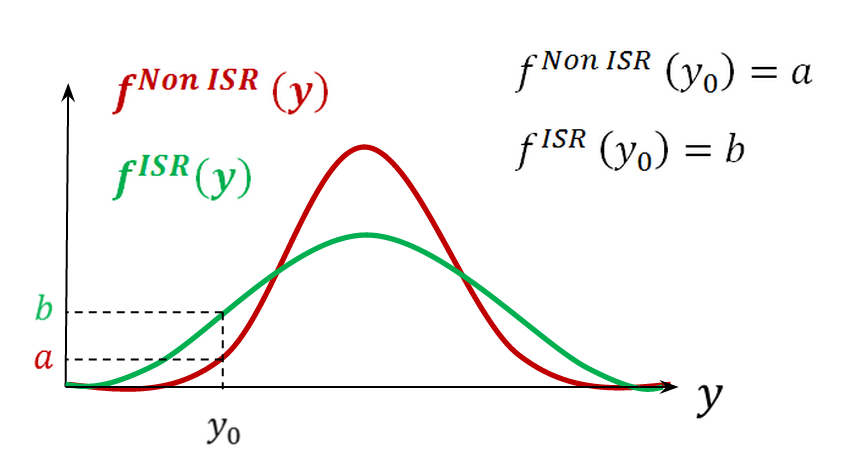
\includegraphics[width=0.7\linewidth]{./Imgs_article/Prob_ISR_Non}
\caption[Probability distributions ISR - Non ISR]{Probability distributions of a variable that distinguishes between ISR and Non ISR jets}
\label{fig:Prob_ISR_Non}
\end{figure}

The difference between both distributions could be used to write the probability of such jet being
ISR or not. In fact, the probability of being ISR should be proportional to the ISR distribution
function at the measurement. Likewise, the probability of being non ISR should be proportional to
the Non ISR distribution function:

\begin{equation} \label{Prob_ISR_1}
P^{ISR}(y_0) \propto f^{ISR}(y_0),
\end{equation}
\begin{equation} \label{Prob_Non_ISR_1}
P^{Non\ ISR}(y_0) \propto f^{Non\ ISR}(y_0).
\end{equation}

In addition to the information offered by the density functions, another important 
consideration to take into account is the \textit{apriori} probability of being ISR. If just one
jet in the event is ISR, the \textit{apriori} probability of any jet being ISR is:

\begin{equation} \label{Prob_ISR_2}
P^{ISR}_{apriori}(y_0) = 1/N_j,
\end{equation}

and similarly, the \textit{apriori} probability of any jet being Non ISR is:

\begin{equation} \label{Prob_Non_ISR_2}
P^{Non\ ISR}_{apriori}(y_0) = \frac{N_j-1}{N_j}.
\end{equation}

Combining both 

This sample document demonstrates proper use of REV\TeX~4.1 (and
\LaTeXe) in mansucripts prepared for submission to APS
journals. Further information can be found in the REV\TeX~4.1
documentation included in the distribution or available at
\url{http://authors.aps.org/revtex4/}.

When commands are referred to in this example file, they are always
shown with their required arguments, using normal \TeX{} format. In
this format, \verb+#1+, \verb+#2+, etc. stand for required
author-supplied arguments to commands. For example, in
\verb+\section{#1}+ the \verb+#1+ stands for the title text of the
author's section heading, and in \verb+\title{#1}+ the \verb+#1+
stands for the title text of the paper.

Line breaks in section headings at all levels can be introduced using
\textbackslash\textbackslash. A blank input line tells \TeX\ that the
paragraph has ended. Note that top-level section headings are
automatically uppercased. If a specific letter or word should appear in
lowercase instead, you must escape it using \verb+\lowercase{#1}+ as
in the word ``via'' above.

\subsection{\label{sec:level2}Second-level heading: Formatting}

This file may be formatted in either the \texttt{preprint} or
\texttt{reprint} style. \texttt{reprint} format mimics final journal output. 
Either format may be used for submission purposes. \texttt{letter} sized paper should
be used when submitting to APS journals.

\subsubsection{Wide text (A level-3 head)}
The \texttt{widetext} environment will make the text the width of the
full page, as on page~\pageref{eq:wideeq}. (Note the use the
\verb+\pageref{#1}+ command to refer to the page number.) 
\paragraph{Note (Fourth-level head is run in)}
The width-changing commands only take effect in two-column formatting. 
There is no effect if text is in a single column.

\subsection{\label{sec:citeref}Citations and References}
A citation in text uses the command \verb+\cite{#1}+ or
\verb+\onlinecite{#1}+ and refers to an entry in the bibliography. 
An entry in the bibliography is a reference to another document.

\subsubsection{Citations}
Because REV\TeX\ uses the \verb+natbib+ package of Patrick Daly, 
the entire repertoire of commands in that package are available for your document;
see the \verb+natbib+ documentation for further details. Please note that
REV\TeX\ requires version 8.31a or later of \verb+natbib+.

\paragraph{Syntax}
The argument of \verb+\cite+ may be a single \emph{key}, 
or may consist of a comma-separated list of keys.
The citation \emph{key} may contain 
letters, numbers, the dash (-) character, or the period (.) character. 
New with natbib 8.3 is an extension to the syntax that allows for 
a star (*) form and two optional arguments on the citation key itself.
The syntax of the \verb+\cite+ command is thus (informally stated)
\begin{quotation}\flushleft\leftskip1em
\verb+\cite+ \verb+{+ \emph{key} \verb+}+, or\\
\verb+\cite+ \verb+{+ \emph{optarg+key} \verb+}+, or\\
\verb+\cite+ \verb+{+ \emph{optarg+key} \verb+,+ \emph{optarg+key}\ldots \verb+}+,
\end{quotation}\noindent
where \emph{optarg+key} signifies 
\begin{quotation}\flushleft\leftskip1em
\emph{key}, or\\
\texttt{*}\emph{key}, or\\
\texttt{[}\emph{pre}\texttt{]}\emph{key}, or\\
\texttt{[}\emph{pre}\texttt{]}\texttt{[}\emph{post}\texttt{]}\emph{key}, or even\\
\texttt{*}\texttt{[}\emph{pre}\texttt{]}\texttt{[}\emph{post}\texttt{]}\emph{key}.
\end{quotation}\noindent
where \emph{pre} and \emph{post} is whatever text you wish to place 
at the beginning and end, respectively, of the bibliographic reference
(see Ref.~[\onlinecite{witten2001}] and the two under Ref.~[\onlinecite{feyn54}]).
(Keep in mind that no automatic space or punctuation is applied.)
It is highly recommended that you put the entire \emph{pre} or \emph{post} portion 
within its own set of braces, for example: 
\verb+\cite+ \verb+{+ \texttt{[} \verb+{+\emph{text}\verb+}+\texttt{]}\emph{key}\verb+}+.
The extra set of braces will keep \LaTeX\ out of trouble if your \emph{text} contains the comma (,) character.

The star (*) modifier to the \emph{key} signifies that the reference is to be 
merged with the previous reference into a single bibliographic entry, 
a common idiom in APS and AIP articles (see below, Ref.~[\onlinecite{epr}]). 
When references are merged in this way, they are separated by a semicolon instead of 
the period (full stop) that would otherwise appear.

\paragraph{Eliding repeated information}
When a reference is merged, some of its fields may be elided: for example, 
when the author matches that of the previous reference, it is omitted. 
If both author and journal match, both are omitted.
If the journal matches, but the author does not, the journal is replaced by \emph{ibid.},
as exemplified by Ref.~[\onlinecite{epr}]. 
These rules embody common editorial practice in APS and AIP journals and will only
be in effect if the markup features of the APS and AIP Bib\TeX\ styles is employed.

\paragraph{The options of the cite command itself}
Please note that optional arguments to the \emph{key} change the reference in the bibliography, 
not the citation in the body of the document. 
For the latter, use the optional arguments of the \verb+\cite+ command itself:
\verb+\cite+ \texttt{*}\allowbreak
\texttt{[}\emph{pre-cite}\texttt{]}\allowbreak
\texttt{[}\emph{post-cite}\texttt{]}\allowbreak
\verb+{+\emph{key-list}\verb+}+.

\end{document}
%
% ****** End of file apssamp.tex ******
